\documentclass[a4paper]{book}
\usepackage[margin=1in]{geometry}
\usepackage[T1]{fontenc}
\usepackage[utf8]{inputenc}
\usepackage[hidelinks]{hyperref}
\usepackage{amsmath}
\usepackage{amssymb}
\usepackage{enumerate}
\usepackage{setspace}
\usepackage{listings}
\usepackage{xcolor}
\usepackage{amsthm}
\usepackage{xspace}
\usepackage{adjustbox}
\usepackage{booktabs} 
\usepackage{array}    
\usepackage{adjustbox} 
\usepackage{colortbl}
\usepackage{graphicx}
\usepackage{ocgx2}
\usepackage{lipsum}


% Configuration pour les listings de code
\definecolor{codebg}{RGB}{245,245,245}
\lstset{
    backgroundcolor=\color{codebg},
    basicstyle=\ttfamily\small,
    frame=single,
    breaklines=true,
    columns=fullflexible,
    keywordstyle=\color{blue},
    commentstyle=\color{gray},
    stringstyle=\color{orange},
    showstringspaces=false
}
\setstretch{1.15}

%----- TITLE PAGE INFO -----%
\title{\Huge \textbf{Spanning Tree Protocol (STP) Workbook}\\
       \Large Fundamentals, Variants, Tuning, and Practical Labs}
\author{\Large Written for Networking Students and Professionals}
\date{\today}

\begin{document}

%----- MODERN TITLE PAGE -----%
\begin{titlepage}
    \centering
    \vspace*{4cm}
    {\Huge \textbf{Spanning Tree Protocol (STP) Workbook}\par}
    \vspace{0.8cm}
    {\Large A Hands-On Guide to PVST+, RSTP, and MSTP\par}
    \vspace{0.3cm}
    \rule{0.9\textwidth}{1pt}
    
    \vspace{0.6cm}
    {\large \textbf{Mehdi JAFARI ZADEH}}\par
    \vspace{0.3cm}

    
    \vfill
    \textbf{Date:} \today
    \vspace{2cm}
\end{titlepage}


\tableofcontents
\newpage

%------------------------------------------------------
% Chapter 1: STP Introduction
%------------------------------------------------------
\chapter{Spanning Tree Protocol (STP)}

\section*{STP Introduction}

Spanning Tree Protocol (STP) is essential for preventing broadcast storms and loops in switched networks with redundant paths. In this section, we'll cover the purpose of STP, its importance in maintaining a loop-free topology, and an overview of how it dynamically reconfigures the network when changes occur. This foundation sets the stage for understanding how STP supports network reliability and resilience.

\section*{Root Bridge}
The Root Bridge is the central reference point in the STP topology. It is elected based on the lowest bridge ID, which is a combination of the bridge priority and MAC address. All other switches in the network compute the best path back to the Root Bridge. Understanding how the Root Bridge is selected is crucial because it directly influences the network's spanning tree structure and the flow of data through the network.

\section*{STP Root Port, Designated Port}
Within each switch (except for the Root Bridge), the Root Port is the interface that offers the best path to the Root Bridge, based on the lowest path cost. On each network segment, the Designated Port is the switch port that has the best path to the Root Bridge and is responsible for forwarding traffic toward it. Together, these port roles determine the active topology of the network by ensuring there is only one active path between any two network devices, thereby preventing loops.


\begin{figure}[h]
    \centering
    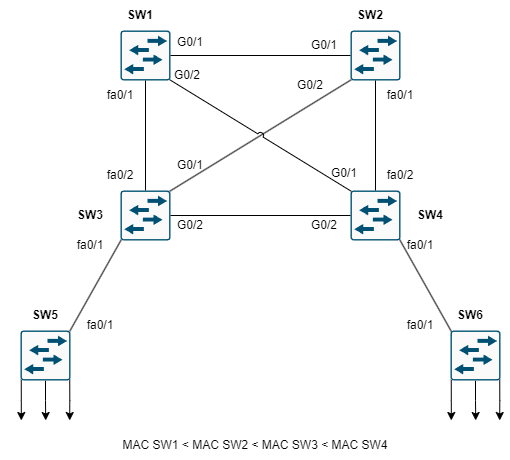
\includegraphics[width=0.9\textwidth]{img/stp01.png}
    \caption{\textit{}}
\end{figure}

\subsection*{Network Topology Overview}
In this exercise, you will work with the network topology as described below. The switches (SW1 to SW6) are connected as Figure 1.1.



The MAC addresses of the switches are as follows:
\begin{center}
    {MAC SW1 $<$ MAC SW2 $<$ MAC SW3 $<$ MAC SW4 $<$ MAC SW6 $<$ MAC SW6}
\end{center}
This means \textbf{SW1} has the lowest MAC address and \textbf{SW6} has the highest.

\section*{Step-by-Step Tasks}

\begin{enumerate}
    \item \textbf{Switch STP Mode to Traditional STP} \\
    Change the STP mode on all switches to \textbf{traditional STP (IEEE 802.1D)}. 
    
    
    
    \item \textbf{Disable Unused Interfaces} \\
    Turn off any extra or unused interfaces to prevent unnecessary loops.

    
    \item \textbf{Set Links to Point-to-Point Mode} \\
    Configure all links between switches as \textbf{Point-to-Point (P2P)} to optimize STP convergence.

    
    \item \textbf{Verify Bridge IDs} \\
    Check the \textbf{Bridge ID} for each switch to see how STP will select the Root Bridge.

    
    \item \textbf{Predict the Root Bridge} \\
    Based on the MAC addresses provided (\textbf{SW1 $<$ SW2 $<$ SW3 $<$ SW4 $<$ SW5 $<$ SW6}), estimate which switch will become the Root Bridge.
    \begin{itemize}
        \item \textit{Question:} Which switch is likely to be the Root Bridge and why?
    \end{itemize}
    
    \item \textbf{Change the Root Bridge by Adjusting Priority} \\
    Modify the \textbf{priority} settings so that the switch identified in the diagram becomes the Root Bridge.
    \begin{itemize}
        
        \item \textit{Note:} Lower priority values increase the chance of a switch becoming the Root Bridge.
    \end{itemize}
    
    \item \textbf{Calculate Path Costs for Active Ports} \\
    For each non-root switch, \textbf{calculate the cost} of paths to the Root Bridge based on link speeds. Use standard STP cost values:
    \begin{itemize}
        \item Gigabit Ethernet (1 Gbps) = 4
        \item Fast Ethernet (100 Mbps) = 19
    \end{itemize}
    
    \item \textbf{Estimate Root Ports} \\
    Identify the \textbf{Root Port} on each non-root switch. This is the port with the lowest path cost to the Root Bridge.
    \begin{itemize}
        \item \textit{Question:} Which port will be the Root Port on SW2, SW3, SW4, SW5, and SW6?
    \end{itemize}
    
    \item \textbf{How Many Root Bridges Are There in a Network?}
    \begin{itemize}
        \item \textit{Question:} In any given STP-enabled network, how many Root Bridges can exist?
    \end{itemize}
    
    \item \textbf{How Many Root Ports Are There in a Network?}
    \begin{itemize}
        \item \textit{Question:} In any given STP-enabled network, how many Root Port can exist?
    \end{itemize}


    \item \textbf{How Many Designated Ports (DP) Are in the Topology?}
    \begin{itemize}
        \item \textit{Question:} In any STP-enabled topology, how many Designated Ports (DP) will there be?
    \end{itemize}

    \item \textbf{Estimate the Designated Ports on Each Switch}
    \begin{itemize}
        \item Before using any commands, predict which ports will be Designated Ports on each switch in the topology. 
    \end{itemize}

    \item \textbf{Verify Designated Ports Using Commands}

    \item \textbf{Are All Root Bridge Ports Designated Ports?}
    \begin{itemize}
        \item \textit{Question:} Based on your observations, can you conclude that all ports on the Root Bridge are Designated Ports?
    \end{itemize}

    \item \textbf{Change the Port Cost of G0/2 on SW4}
    \begin{itemize}
        \item Modify the path cost of interface G0/2 on SW4 to 15. This will influence STP’s decision on which path to use. 
    \end{itemize}

    \begin{figure}[h]
        \centering
        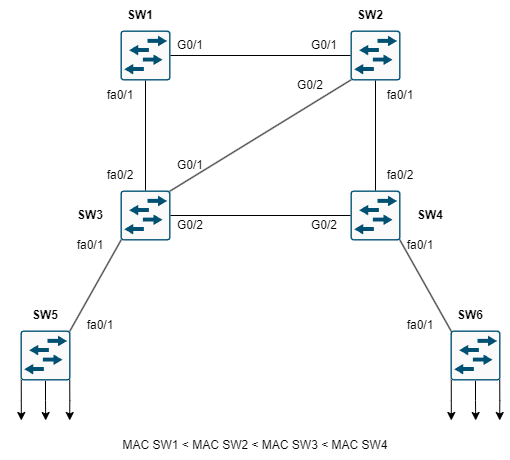
\includegraphics[width=0.9\textwidth]{img/stp02.png}
        \caption{\textit{}}
    \end{figure}
    \newpage


    \item \textbf{Predict the New Root Port on SW4 After Link Removal}
    \begin{itemize}
        \item If you remove the link connected to G0/1 on SW4 (Figure 1.2), which port will become the new Root Port? Explain your reasoning based on path costs and STP rules.
        \item \textit{Hint:} Consider which remaining port on SW4 has the lowest cost path to the Root Bridge.
    \end{itemize}

    \item \textbf{Identify Root Ports with SW1 as the Root Bridge}
    \begin{itemize}
        \item In this topology, assuming SW1 is the Root Bridge, identify the Root Ports on the other switches (SW2, SW3, SW4, SW5, and SW6).
 
    \end{itemize}

    \item \textbf{Change the Port ID to Influence Link Selection}
    \begin{itemize}
        \item STP uses Port IDs as a tie-breaker when path costs are equal. By adjusting the Port Priority (which is part of the Port ID), you can influence which link STP selects as the active path.
        \item \textit{Task:} Change the Port Priority of specific interfaces to modify STP’s link selection.
    \end{itemize}
    
\end{enumerate}

\newpage
\section*{Additional exercises}
\subsection*{Draw the Active Topology for Each Scenario}


\begin{figure}[h]
    \centering
    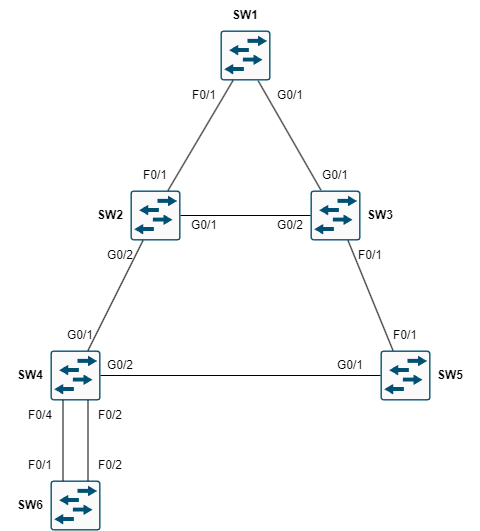
\includegraphics[width=0.4\textwidth]{img/stp03.png}
    \caption{\textit{}}
\end{figure}

\begin{figure}[h]
    \centering
    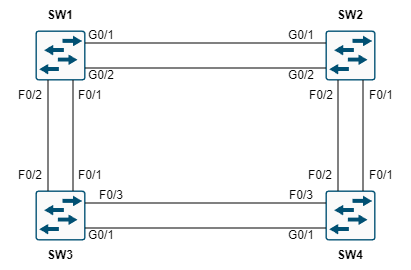
\includegraphics[width=0.4\textwidth]{img/stp04.png}
    \caption{\textit{}}
\end{figure}

\begin{figure}[h]
    \centering
    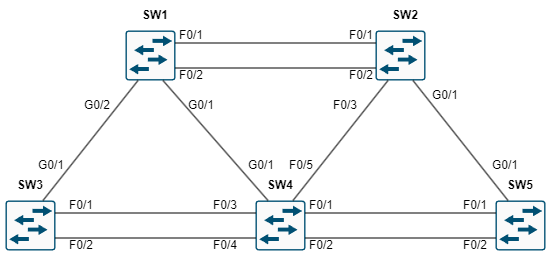
\includegraphics[width=0.5\textwidth]{img/stp05.png}
    \caption{\textit{}}
\end{figure}

%------------------------------------------------------
% Chapter 2: STP Root Bridge
%------------------------------------------------------
\chapter{PVST (Per-VLAN Spanning Tree)}

\section*{What is PVST?}
Per-VLAN Spanning Tree (PVST) is a version of the Spanning Tree Protocol (STP) that creates a separate spanning tree instance for each VLAN in the network. This allows for better load balancing and more efficient use of network resources, as different VLANs can have different root bridges and forwarding paths.


\section*{Key Features of PVST:}
\begin{enumerate}
    \item \textbf{Separate Spanning Tree per VLAN:}
    \newline
    Each VLAN runs its own independent instance of STP, meaning the topology can be optimized differently for each VLAN.
    \item \textbf{Improved Load Balancing:}
    
    By assigning different root bridges to different VLANs, PVST allows traffic to be distributed across multiple switches, reducing congestion and improving performance.
    
    \item Root Bridge Election per VLANCompatibility with Cisco Devices:
    
    VST is a Cisco proprietary protocol and is typically used in Cisco environments. It is based on the original IEEE 802.1D standard but with VLAN-specific enhancements.
    \item \textbf{Uses Common STP Concepts:}
    
    PVST uses the same roles and states as traditional STP:
    \begin{itemize}
        \item Root Bridge
        \item Root Port (RP)
        \item Designated Port (DP)
        \item Blocked Port
    \end{itemize}
\end{enumerate}

\section*{How PVST Works:}
\begin{itemize}
    \item \textbf{Root Bridge Election per VLAN:}
    
    Each VLAN elects its own Root Bridge based on the lowest Bridge ID (priority + MAC address). This allows different switches to act as the Root Bridge for different VLANs.

    \item \textbf{Port Roles and Path Selection:}
    
    For each VLAN, PVST determines the Root Ports and Designated Ports independently, which results in different forwarding paths for different VLANs.
\end{itemize}


\section*{Benefits of PVST:}
\begin{itemize}
    \item \textbf{Flexibility:} Allows network administrators to optimize traffic flow for each VLAN.
    \item \textbf{Load Balancing:} Distributes traffic across multiple links by having different root bridges for different VLANs.
    \item \textbf{Faster Convergence:} PVST+ (an enhanced version) offers faster convergence times compared to traditional STP.

\end{itemize}

\newpage

\chapter{PVST+ Lab Exercise: VLAN-Based Root Bridge Configuration}

\section*{Network Topology Overview}
In this scenario, you will configure \textbf{PVST+ (Per-VLAN Spanning Tree Plus)}, which allows separate spanning tree instances for each VLAN. The network consists of three switches (\textbf{SW1}, \textbf{SW2}, and \textbf{SW3}) and multiple VLANs with end devices connected to each switch.


\begin{figure}[h]
    \centering
    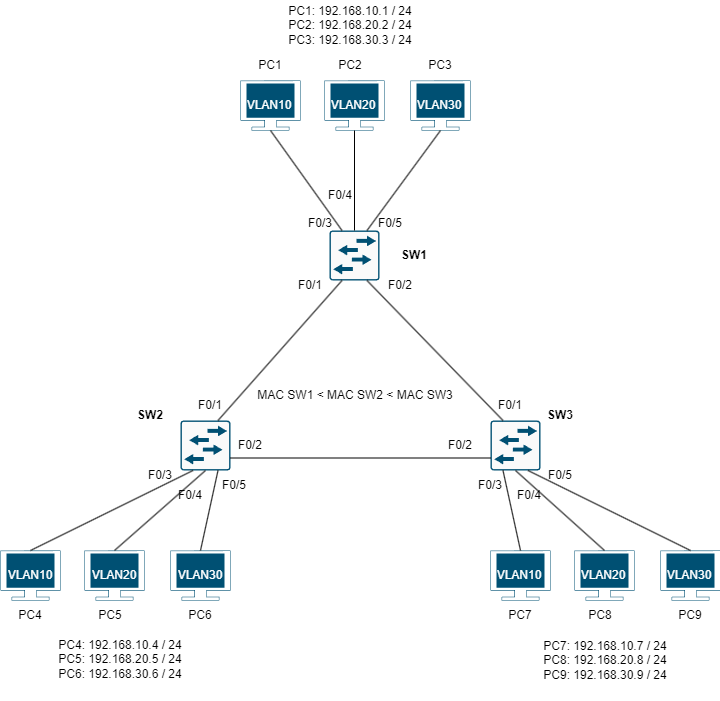
\includegraphics[width=0.8\textwidth]{img/pvst01.png}
    \caption{\textit{}}
\end{figure}


\begin{itemize}
    \item \textbf{MAC Address Order:} \\
    \textbf{MAC SW1 $<$ MAC SW2 $<$ MAC SW3} \\
    (SW1 has the lowest MAC address.)
    
    \item \textbf{VLANs and Devices:}
    \begin{itemize}
        \item \textbf{VLAN 10:} PC1, PC4, PC7
        \item \textbf{VLAN 20:} PC2, PC5, PC8
        \item \textbf{VLAN 30:} PC3, PC6, PC9
    \end{itemize}
\end{itemize}

\section*{Step-by-Step Configuration Tasks}

\begin{enumerate}

    \item \textbf{Set Inter-Switch Links to Trunk Mode} \\
    Configure the links between the switches (\textbf{SW1, SW2, SW3}) to operate in \textbf{trunk mode} to allow VLAN traffic to pass through.
    
    
    \item \textbf{Verify Current STP Status} \\
    Before making further changes, \textbf{check the current STP status} to see how the network has chosen the Root Bridge for each VLAN.
    

    \item \textbf{Enable VTP on All Switches} \\
    Configure \textbf{VTP (VLAN Trunking Protocol)} to manage VLANs centrally.
    
    \textbf{VTP Settings:}
    \begin{itemize}
        \item \textbf{Domain Name:} \texttt{network}
        \item \textbf{Version:} \texttt{2}
        \item \textbf{Password:} \texttt{CCNP}
    \end{itemize}


    - SW1 Configuration (VTP Master/Server):


    - SW2 and SW3 Configuration (VTP Clients):


    \item \textbf{Create VLANs 10, 20, and 30 on SW1 (VTP Server)} \\
    Since \textbf{SW1} is the VTP Server, create the VLANs here, and they will propagate to \textbf{SW2} and \textbf{SW3}.
    

    \item \textbf{Verify STP Status After VLAN Creation} \\
    After setting up VTP and VLANs, check how \textbf{PVST} has adjusted the spanning tree roles.

\end{enumerate}

\section*{PVST Root Bridge Configuration Per VLAN}

\begin{enumerate}

    \item \textbf{Set Root Bridges for Each VLAN Using PVST+} \\
    Configure different \textbf{Root Bridges} for each VLAN to optimize traffic flow:

    \begin{itemize}
        \item \textbf{VLAN 10 Root Bridge:} Set \textbf{SW1} as the Root Bridge.
        \item \textbf{VLAN 20 Root Bridge:} Set \textbf{SW2} as the Root Bridge.
        \item \textbf{VLAN 30 Root Bridge:} Set \textbf{SW3} as the Root Bridge.
    \end{itemize}

 

    - SW1 (Root for VLAN 10):


    - SW2 (Root for VLAN 20):


    - SW3 (Root for VLAN 30):


    \textit{Note:} A lower priority value increases the likelihood of a switch becoming the Root Bridge. The default is 32768.

    \item \textbf{Verify STP Status After Root Bridge Configuration} \\
    After configuring the Root Bridges for each VLAN, verify that the changes were applied correctly.


    \textbf{Question:}
    \begin{enumerate}
        \item Which switch is now the Root Bridge for each VLAN?
        \item How did the Root Ports and Designated Ports change across the network?
    \end{enumerate}
\newpage
    \item \textbf{Draw the active topology of each violin.} \\
    - SW1 (Root for VLAN 10):


    - SW2 (Root for VLAN 20):


    - SW3 (Root for VLAN 30):
    \begin{figure}[h]
        \centering
        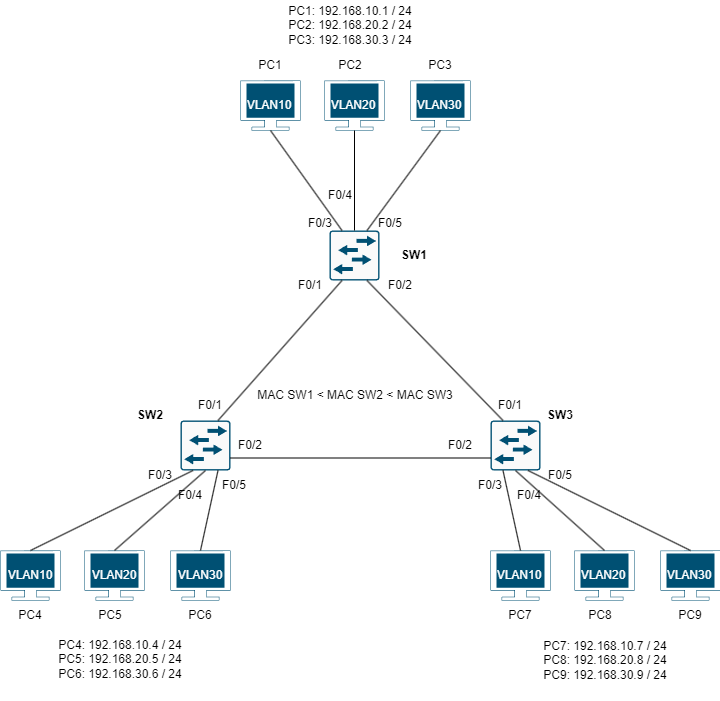
\includegraphics[width=0.8\textwidth]{img/pvst01.png}
        \caption{\textit{}}
    \end{figure}
\end{enumerate}


\newpage

\section*{Configure PortFast for End Devices}

\begin{enumerate}
    \item \textbf{Enable PortFast on All PC Ports} \\
    PortFast allows end devices (like PCs) to bypass STP's listening and learning states, enabling faster connections.

    \textit{Task:} Configure \textbf{PortFast} on interfaces connected to PCs (e.g., \textbf{F0/3}, \textbf{F0/4}, \textbf{F0/5} on SW1).

    \item \textbf{Verify Connectivity Between PC2 and PC3} \\
    \textit{Task:} Test the connection between \textbf{PC2 (192.168.20.2)} and \textbf{PC3 (192.168.30.3)} using the \textbf{ping} command.


    \item \textbf{Enable Debugging on SW3} \\
    Monitor STP behavior during topology changes.

    \textit{Task:} Turn on STP debugging on \textbf{SW3}.

    \item \textbf{Shut Down Interfaces to Trigger Topology Changes} \\
    Simulate link failures by shutting down specific interfaces:

    \textit{Task:} Shut down \textbf{F0/1} on \textbf{SW3} and \textbf{F0/2} on \textbf{SW1}:


    \item \textbf{Observe and Estimate New Topology} \\
    After shutting down the interfaces:

    \textit{Task:} Check the \textbf{new port roles} and \textbf{STP state} using:


    \textbf{Question:} Which ports have become \textbf{Root Ports} or \textbf{Designated Ports}? Identify if any ports are now \textbf{Blocked}.

    \item \textbf{Restore the Network to Its Original State} \\
    Re-enable the interfaces to bring the network back to its initial state.

    \textit{Task:}  Turn on \textbf{F0/1} on \textbf{SW3} and \textbf{F0/2} on \textbf{SW1}:


    \item \textbf{Reduce Network Diameter for Faster Convergence} \\
    The \textbf{network diameter} defines the maximum number of switches a BPDU can pass through. Reducing it speeds up convergence.

    \textit{Task:} Reduce the \textbf{network diameter} from the default \textbf{7} to \textbf{2}.

    \item \textbf{Check Forward Delay and Max Age Timers} \\
    STP uses these timers to control how long switches stay in different states during convergence.

    \textit{Task:} Verify \textbf{Forward Delay} and \textbf{Max Age} settings:

    \item \textbf{Enable UplinkFast on SW2 for Faster Recovery} \\
    \textbf{UplinkFast} speeds up STP convergence when a primary link fails by immediately switching to a backup link.

    \textit{Task:} Enable \textbf{UplinkFast} on \textbf{SW2}:

    \item \textbf{Set Max-Update-Rate to 100 Packets per Second} \\
    Limit the number of update packets sent per second to prevent excessive flooding during topology changes.

    \textit{Task:} Set \textbf{max-update-rate} to \textbf{100 packets/sec}:


    \item \textbf{Verify Uplink Status on SW2} \\
    \textit{Task:} Check if \textbf{UplinkFast} is working correctly:

\end{enumerate}

\section*{Discussion Questions}

\begin{enumerate}
    \item How did reducing the network diameter impact convergence speed?
    \item After enabling UplinkFast, how quickly did SW2 recover from link failures?
\end{enumerate}
\chapter{Protecting the Spanning Tree Protocol (STP) Topology}


\noindent The \textbf{Spanning Tree Protocol (STP)} is crucial for maintaining a loop-free and stable Layer 2 network topology. However, without proper safeguards, STP can become vulnerable to misconfigurations or malicious attacks, potentially leading to network loops, instability, or even downtime. To enhance the security and stability of the STP topology, network administrators can implement various protection mechanisms, including \textbf{BPDU Guard}, \textbf{Root Guard}, \textbf{BPDU Filter}, \textbf{Loop Guard}, and \textbf{UDLD (Unidirectional Link Detection)}. These features help prevent unauthorized devices from influencing STP operations, detect unidirectional links, and ensure consistent network behavior.

\section*{BPDU Guard}

\textbf{Bridge Protocol Data Units (BPDUs)} are essential messages exchanged between switches to maintain the STP topology. \textbf{BPDU Guard} is a protective feature designed to secure \textbf{PortFast}-enabled ports, which are typically connected to end devices like computers or printers. Since these ports bypass STP’s usual listening and learning states to achieve faster connectivity, receiving BPDUs on them could indicate a misconfiguration or an attack (such as connecting a rogue switch).

When \textbf{BPDU Guard} is enabled and a BPDU is received on a PortFast port, the switch immediately \textbf{disables} the port by placing it into an \textbf{err-disabled} (error-disabled) state. This action prevents potential network loops and unauthorized participation in the STP topology. BPDU Guard is particularly useful in access layer switches where end devices should never send BPDUs.

\section*{Root Guard}

The \textbf{Root Bridge} plays a central role in STP, determining the best loop-free paths for traffic. If an unauthorized switch with a \textbf{lower Bridge ID} (priority + MAC address) is connected to the network, it could inadvertently or maliciously become the Root Bridge, altering the topology and potentially degrading network performance.

\textbf{Root Guard} prevents this by restricting specific ports from becoming Root Ports. When enabled on a port, if a superior BPDU (indicating a better Root Bridge) is received, the port is placed into a \textbf{root-inconsistent} state, effectively blocking it from influencing the Root Bridge election. Once the superior BPDUs stop, the port automatically returns to normal operation. Root Guard is typically applied on ports where no upstream Root Bridge should be allowed, such as those connecting to access layer switches.

\section*{BPDU Filter}

While \textbf{BPDU Guard} reacts to unexpected BPDUs, \textbf{BPDU Filter} prevents BPDUs from being sent or received on specific ports altogether. This feature can be applied globally or on a per-port basis:

\begin{itemize}
    \item \textbf{Globally:} BPDU Filter allows initial BPDUs to be sent when a port comes up but suppresses further BPDU exchange, making the port behave as if STP is disabled.
    \item \textbf{Per-Port:} When applied directly to a port, BPDU Filter prevents all BPDUs from being sent or received, effectively removing the port from STP participation.
\end{itemize}

\textbf{Caution:} Improper use of BPDU Filter can lead to \textbf{network loops}, as the port is unaware of STP topology changes. It should be used in controlled environments where the risk of loops is minimal.

\section*{Loop Guard}

\textbf{Loop Guard} is designed to prevent loops caused by \textbf{unidirectional link failures} in STP. In normal operation, a port in a \textbf{blocking} or \textbf{root port} state relies on receiving BPDUs from neighboring switches to maintain its status. If BPDUs unexpectedly stop arriving due to a failure, the port might incorrectly transition to the \textbf{forwarding} state, creating a loop.

When \textbf{Loop Guard} is enabled, if a port stops receiving BPDUs on a \textbf{non-designated port} (i.e., a blocking or root port), the port enters a \textbf{loop-inconsistent} state instead of transitioning to forwarding. This proactive measure prevents loops by ensuring ports stay in a safe state until the issue is resolved. Loop Guard is particularly useful on redundant links where unidirectional failures could silently cause loops.

\section*{UDLD (Unidirectional Link Detection)}

\textbf{Unidirectional Link Detection (UDLD)} is a Layer 2 protocol that detects unidirectional physical link failures, which can lead to network loops or black holes. Such failures occur when traffic flows in one direction but not the other, often due to fiber optic issues, hardware faults, or misconfigurations.

UDLD operates by exchanging \textbf{hello packets} between devices on both ends of a link. If one device stops receiving these packets while still sending its own, UDLD detects the inconsistency. Depending on the mode:
\begin{itemize}
    \item In \textbf{normal mode}, UDLD alerts administrators but does not take immediate action.
    \item In \textbf{aggressive mode}, UDLD automatically \textbf{disables} the affected port to prevent potential loops.
\end{itemize}

UDLD is particularly important in fiber optic networks, where physical link issues might not be immediately evident.

\section*{Conclusion}

Securing the \textbf{Spanning Tree Protocol} topology is essential for maintaining a reliable and stable network. Features like \textbf{BPDU Guard} and \textbf{Root Guard} prevent unauthorized devices from influencing the STP topology, while \textbf{BPDU Filter} and \textbf{Loop Guard} ensure proper BPDU handling and loop prevention. Additionally, \textbf{UDLD} plays a critical role in detecting and mitigating unidirectional link failures. By implementing these protective mechanisms, network administrators can significantly enhance the robustness and resilience of their Layer 2 networks, reducing the risk of outages, loops, and other network disruptions.


\newpage
\section*{Lab Exercises: Protecting the Spanning Tree Protocol Topology}

\begin{figure}[h]
    \centering
    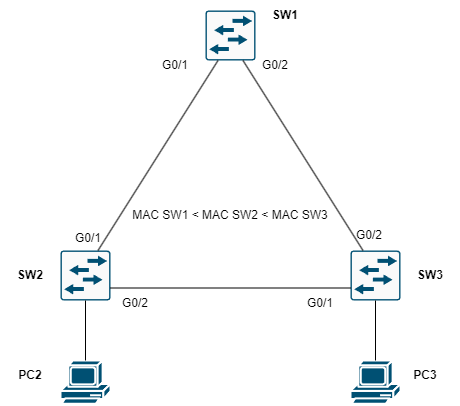
\includegraphics[width=0.8\textwidth]{img/STPConvergence01.png}
    \caption{\textit{}}
\end{figure}

\subsection*{Network Topology Overview:}

\begin{itemize}
    \item \textbf{SW1} is connected to \textbf{SW2} and \textbf{SW3}.
    \item \textbf{SW2} is connected to \textbf{PC2} and has a direct link to \textbf{SW3}.
    \item \textbf{SW3} is connected to \textbf{PC3}.
    \item \textbf{MAC Address Order:} \\
    \textbf{MAC SW1 $<$ MAC SW2 $<$ MAC SW3} \\
    (SW1 has the lowest MAC address and will likely become the Root Bridge unless configured otherwise.)
\end{itemize}

\subsection*{Configuring BPDU Guard}

\textbf{Objective:} Protect access ports from unauthorized devices sending BPDUs, which could cause topology changes.

\begin{enumerate} 
    \item \textbf{Enable BPDU Guard on Access Ports (Connected to PCs):} \\
    Since \textbf{PC2} and \textbf{PC3} are end devices, their interfaces should not receive BPDUs. If a BPDU is received, BPDU Guard will shut down the port to prevent loops.

    On SW2 (Port connected to PC2) and SW3 (Port connected to PC3):


    \item \textbf{Test the Configuration:} \\
    Connect a switch (instead of a PC) to \textbf{G0/2} on \textbf{SW2} and send BPDUs.

    \textbf{Expected Result:} The port should move to an \textbf{err-disabled} state. Verify using:


    \item \textbf{Recover the Port:}

\end{enumerate}

\subsection*{Configuring Root Guard}

\textbf{Objective:} Prevent unauthorized switches from becoming the Root Bridge.

\begin{enumerate} 
    \item \textbf{Enable Root Guard on Specific Ports:} \\
    To ensure \textbf{SW1} remains the Root Bridge, apply Root Guard on \textbf{SW2} and \textbf{SW3} ports facing other switches.

    On SW2 (Facing SW3) and SW3 (Facing SW2):


    \item \textbf{Test the Configuration:} \\
    Lower the bridge priority on \textbf{SW3} to try to make it the Root Bridge:


    \textit{Expected Result:} The port on \textbf{SW2} connected to \textbf{SW3} should go into a \textbf{root-inconsistent} state, preventing \textbf{SW3} from becoming the Root Bridge.

    \item \textbf{Verify the Root Guard Status:}

\end{enumerate}



Here is some regular text. \\
\vspace{0.5cm}


\switchocg{codeblock}{%
    \color{black}\underline{Click here to reveal the code!}%
}


\begin{ocg}{Code Block}{codeblock}{0}
\vspace{0.5cm}
\begin{lstlisting}
Switch1(config)# 
\end{lstlisting}
\end{ocg}


\section*{Exercise 3: Configuring BPDU Filter}

\textbf{Objective:} Suppress BPDU transmission on specific ports to prevent unnecessary STP participation.

\begin{enumerate} 
    \item \textbf{Enable BPDU Filter on Access Ports (Connected to PCs):}

    \textbf{On SW2 (Port connected to PC2):}
    \begin{verbatim}
interface g0/2
spanning-tree bpdufilter enable
    \end{verbatim}

    \textbf{On SW3 (Port connected to PC3):}
    \begin{verbatim}
interface g0/1
spanning-tree bpdufilter enable
    \end{verbatim}

    \item \textbf{Test the Configuration:} \\
    Verify that BPDUs are not being sent on these interfaces:
    \begin{verbatim}
debug spanning-tree bpdu send
    \end{verbatim}

    \item \textbf{Warning:} \\
    \textbf{BPDU Filter} disables STP on the interface, which can lead to network loops if a switch is accidentally connected.
\end{enumerate}

\section*{Exercise 4: Configuring Loop Guard}

\textbf{Objective:} Prevent loops caused by unidirectional link failures in the STP topology.

\begin{enumerate} 
    \item \textbf{Enable Loop Guard on Non-Designated Ports:} \\
    Loop Guard should be applied to \textbf{root ports} and \textbf{alternate ports} that might stop receiving BPDUs.

    \textbf{On SW2 and SW3 (Ports facing SW1):}
    \begin{verbatim}
interface g0/0
spanning-tree guard loop
    \end{verbatim}

    \item \textbf{Simulate a Unidirectional Link Failure:} \\
    Disconnect the \textbf{TX (Transmit)} fiber cable from \textbf{SW1’s G0/1} while keeping \textbf{RX (Receive)} connected.

    \textbf{Expected Result:} The port on \textbf{SW2} should enter a \textbf{loop-inconsistent} state instead of transitioning to forwarding.

    \item \textbf{Verify Loop Guard Status:}
    \begin{verbatim}
show spanning-tree inconsistentports
    \end{verbatim}
\end{enumerate}

\section*{Exercise 5: Configuring UDLD (Unidirectional Link Detection)}

\textbf{Objective:} Detect and disable unidirectional links to prevent loops.

\begin{enumerate} 
    \item \textbf{Enable UDLD on Fiber Links Between Switches:} \\
    Apply UDLD on the \textbf{G0/1} and \textbf{G0/2} interfaces between switches.

    \textbf{On SW1:}
    \begin{verbatim}
interface range g0/1 - 2
udld aggressive
    \end{verbatim}

    \textbf{On SW2 and SW3 (Interfaces facing SW1):}
    \begin{verbatim}
interface g0/0
udld aggressive
    \end{verbatim}

    \item \textbf{Test UDLD Functionality:} \\
    Disconnect one side of the fiber link (e.g., \textbf{TX} on \textbf{SW1 G0/1}).

    \textbf{Expected Result:} UDLD will detect the unidirectional link and place the port in an \textbf{err-disabled} state.

    \item \textbf{Verify UDLD Status:}
    \begin{verbatim}
show udld interface
    \end{verbatim}

    \item \textbf{Recover UDLD-disabled Ports:}
    \begin{verbatim}
interface g0/1
udld reset
    \end{verbatim}
\end{enumerate}

\section*{Discussion Questions:}

\begin{enumerate} 
    \item What happens when BPDU Guard is triggered? How is this different from BPDU Filter?
    \item How does Root Guard prevent unauthorized topology changes, and in what scenarios would it be most useful?
    \item What is the difference between Loop Guard and UDLD in handling unidirectional link failures?
    \item After enabling UDLD, how quickly did the network detect and respond to a unidirectional failure compared to standard STP behavior?
\end{enumerate}


\end{document}
